\documentclass[10pt,a4paper]{article}
\usepackage{CJKutf8}
\usepackage{url}
\usepackage{caption}
\usepackage{graphicx}
\usepackage{subfigure}
\usepackage{amsmath}
\usepackage{amssymb}
\usepackage{overpic}
\usepackage{enumitem}
\usepackage{amsthm}
\usepackage{geometry}
\usepackage[noend]{algpseudocode}
\usepackage{algorithmicx,algorithm}
\usepackage{hyperref}
\hypersetup{colorlinks=true,
            linkcolor=blue,
            anchorcolor=blue,
            citecolor=blue}
\usepackage{biblatex}
\addbibresource{mybib.bib}
\renewcommand{\baselinestretch}{1.2}
\setcounter{page}{1}
\geometry{left=2.0cm, right=2.0cm, top=1cm, bottom=1.5cm}

\newtheorem{theorem}{Theorem}[section]
\newtheorem{remark}{Remark}[section]
\newtheorem{definition}{Definition}[section]
\newtheorem{lemma}{Lemma}[section]

\begin{document}
\begin{CJK}{UTF8}{gbsn}
\title{Nonlinar compensation algorithm for WDM system in optical fiber}
\author{Xinyu Xiao, Bin Dong, Zhennan Zhou} 
\maketitle
\tableofcontents

\begin{abstract}
In long-haul optical communication systems, compensating nonlinear effects through digital signal processing (DSP) 
is difficult due to intractable interactions between Kerr nonlinearity, chromatic dispersion (CD) and amplified 
spontaneous emission (ASE) noise from inline amplifiers. We constructed a pytorch-based optical fiber communication 
system including Tra  nsmitter, fiber channel model and receiver. We design some 
digital back propagation models and test their performence. We get some improvements
compared with some latest work.
\end{abstract}

\section{Communication System}
\subsection{overview}
There are the most important components in  a fiber communication system (see Figure [\ref{flow-chart}]): 
\begin{enumerate}
\item Transmitter: turn a complex symbol sequence to a wave form signal and transmitted to a fiber channel.
$$
\{X_n\}_{n=0}^{N} \rightarrow u(0,t), t\in R^{+}
$$
Where $X_n\in \mathbb{C}$ are the transmmited symbols, $u \in \mathbb{C}$ is the wave form signal. We assume total N symbols here.
\item Fiber channel: evolution the analog signal from $z=0$ to $z=L$.
$$
 u(0,t) \rightarrow u(L,t)
$$
\item Reciever: sampled data points from the received signal $u(L,t)$ and turn this data to a complex symbol sequence. 
$$
u(L,t) \rightarrow \{Y_n\}_{n=0}^{N}
$$ 
where $Y_n \in \mathbb{C}$ is output symbols.
\end{enumerate}
\begin{figure}[ht]
\centering
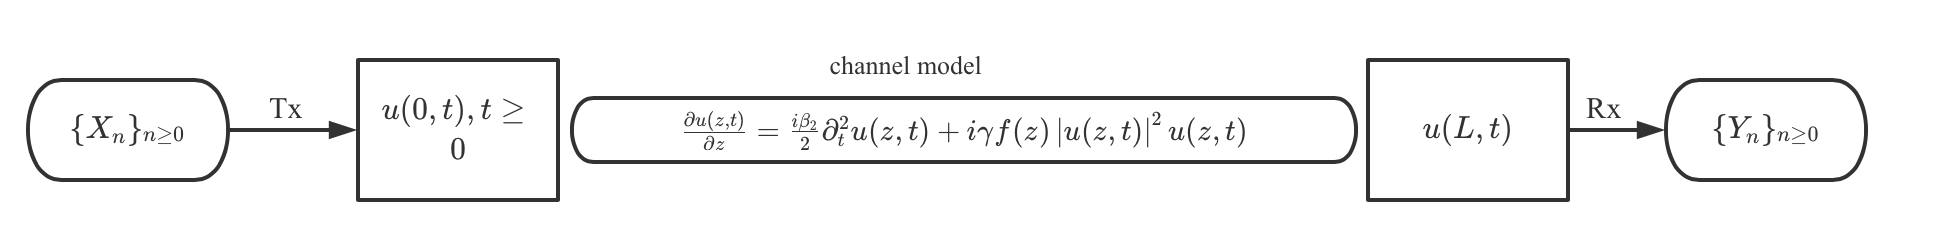
\includegraphics[width=\linewidth]{img/flow-chart.png}
\caption{data flow}
\label{flow-chart}
\end{figure}
Because of the noise in fiber channel, we get a channel conditional probability:
$$
P(Y|X)
$$
where $X = (X_1,X_2,\ldots,X_N)$, $Y=(Y_1,Y_2,\ldots,Y_N)$.\\
\textbf{Our target}
\begin{enumerate}
\item In practice. We want to increase the bit error rate(BER) as much as we can.
$$
BER = Pr(X_n=Y_n)
$$
\item In theorem. We want to know the capacity limit in such a nonlinear communication system.
\begin{align*}
C = \sup\limits_{P(X)} \frac{1}{N}I(X:Y)
\end{align*}
Here $I(X;Y)$ is the mutual information between two random vectors. This formula is the famous Seccond shannon theorem.
\end{enumerate}


\subsection{Transmitter Model}

\begin{equation}\label{Tx}
\left\{
\begin{aligned}
& u(0,t) = \sum_{i=M}^{-M} A_i(0,t) exp(i (\omega_i - \omega_0) t) & t\in [0,T_f]\\
& A_i(0,t) = \sqrt{P_i}\sum_{k=0}^{N-1} x^i_k g(t - kT) \\
\end{aligned}
\right.
\end{equation}
Where $g(t)$ is the Raise-Cosin signal pulse controled by a roll-off parameter $\beta$. Show as formula (\ref{pulse}) and figure (\ref{Raise-Cosin}). $T$ is symbol period and $T_f = N*T$ is the signal length. $P_0$ is the peak power. $x^i_k \in \mathbb{C}$ is complex symbol (See Remark (\ref{4QAM})). $\omega_0$ is the central carrier frenquency.

\begin{remark}\label{4QAM}
[4QAM]
$$
x^k_j \in \mathcal{X} = \{\pm 1 \pm i \}
$$
\begin{figure}[htbp]
\centering
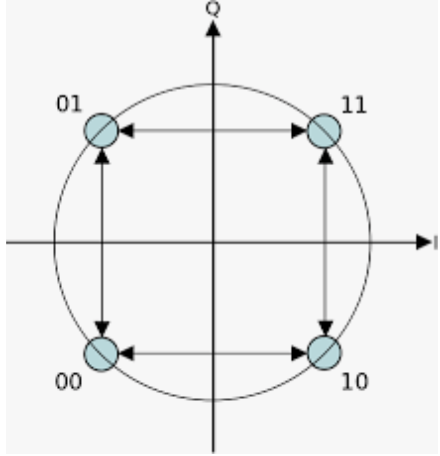
\includegraphics[width=0.2\linewidth]{img/4QAM.png}
\end{figure}
\end{remark}

\begin{equation}\label{pulse}
g(t)=\left\{\begin{array}{ll}
\frac{\pi}{4 T} \operatorname{sinc}\left(\frac{1}{2 \beta}\right), & t=\pm \frac{T}{2 \beta} \\
\frac{1}{T} \operatorname{sinc}\left(\frac{t}{T}\right) \frac{\cos \left(\frac{\pi \beta t}{T}\right)}{1-\left(\frac{2 \beta t}{T}\right)^{2}}, & \text { otherwise }
\end{array}\right.
\end{equation}

\begin{figure}[htbp]
\centering
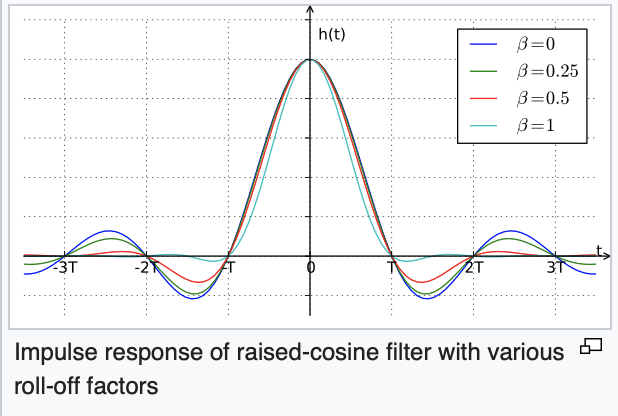
\includegraphics[width=0.3\linewidth]{img/rc_t.png}
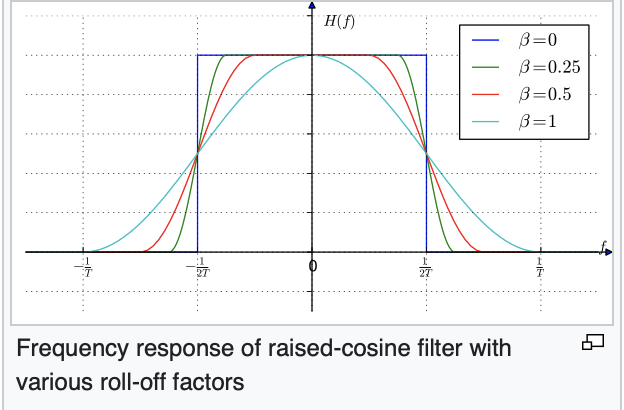
\includegraphics[width=0.3\linewidth]{img/rc_f.png}
\caption{Raise-Cosin signal pulse}
\label{Raise-Cosin}
\end{figure}


\subsection{Fiber model}
\subsubsection{Nonlinear Schrodinger equation model (NLSE)}
\begin{equation}\label{model}
\left\{
\begin{aligned}
& \frac{\partial u(z, t)}{\partial z}=-\frac{\alpha}{2}u(z,t) + \frac{i\beta_2}{2} \frac{\partial^2 u(z,t)}{\partial t^2} + i \gamma \left|u(z, t)\right|^{2} u(z, t) + n(z,t) \\
& u(z,0) = u(z,T_f) \\
& u(0,t) = \sum_{i=M}^{-M} A_i(0,t) exp(i (\omega_i - \omega_0) t) \\
& A_i(0,t) = \sqrt{P_i}\sum_{k=1}^{N} x^i_k g(t - kT) \\
& (z,t) \in [0,L] \times [0,T_f]
\end{aligned}
\right.
\end{equation}
Where $\alpha$,$\beta_2$,$\gamma$ denote attenuation, group velocity dispersion, and fiber nonlinearity coefficient.  $n(z,t)$ is a complex Gaussian noise process with autocorrelation (\ref{noise})(see \cite{path_int}). 
\begin{remark}\label{noise}
[noise term]
\begin{equation}
\left\{
\begin{aligned}
& \left\langle n(z, \omega) \bar{n}\left(z^{\prime}, \omega^{\prime}\right)\right\rangle_{n}=2 \pi \mathcal{Q} \delta\left(\omega-\omega^{\prime}\right) \theta\left(\frac{W^{\prime}}{2}-|\omega|\right) \delta\left(z-z^{\prime}\right) \\
& \left\langle n(z, t) \bar{n}\left(z^{\prime}, t^{\prime}\right)\right\rangle_{n}=\frac{\mathcal{Q}}{\pi\left(t-t^{\prime}\right)} \sin \left(\frac{W^{\prime}\left(t-t^{\prime}\right)}{2}\right) \delta\left(z-z^{\prime}\right)
\end{aligned}
\right.
\end{equation}

Where $\theta(x)$ is Heaviside theta-function. 

\end{remark}


\begin{remark}
[FT]
$$
n(z, \omega)=\int_{-\infty}^{\infty} d t e^{-i \omega t} n(z, t)
$$
\end{remark}



\subsubsection{Couple Nonlinear Schrodinger Equation model (CNLSE)}
Use the WDM initial expression (\ref{WDM initial value}), and neglect FWM terms(when can we neglect this term ?), we can get a simpler model (\ref{CNLSE}).
\begin{equation}\label{WDM initial value}
u(z,t) = \sum_{i=M}^{-M} A_i(z,t) exp(i (\omega_i - \omega_0) t)
\end{equation}

\begin{equation}\label{CNLSE}
\frac{\partial A_i(z, t)}{\partial z}=-\frac{\alpha}{2}A_i(z,t)-\beta_{i1}\frac{\partial A_i(z,t)}{\partial t} + \frac{i\beta_{i2}}{2} \frac{\partial^2 A_i(z,t)}{\partial t^2} + i \gamma \left(|A_i|^{2} + 2\sum_{q\neq i} |A_q|^2\right) A_i(z, t) + n(z,t)
\end{equation}

\subsubsection{Split Step Fourier Method}
To solve the NLSE and CNLSE, we review the classical Split Step Fourier Method(SSFM) .
\begin{figure}[htbp]
\centering
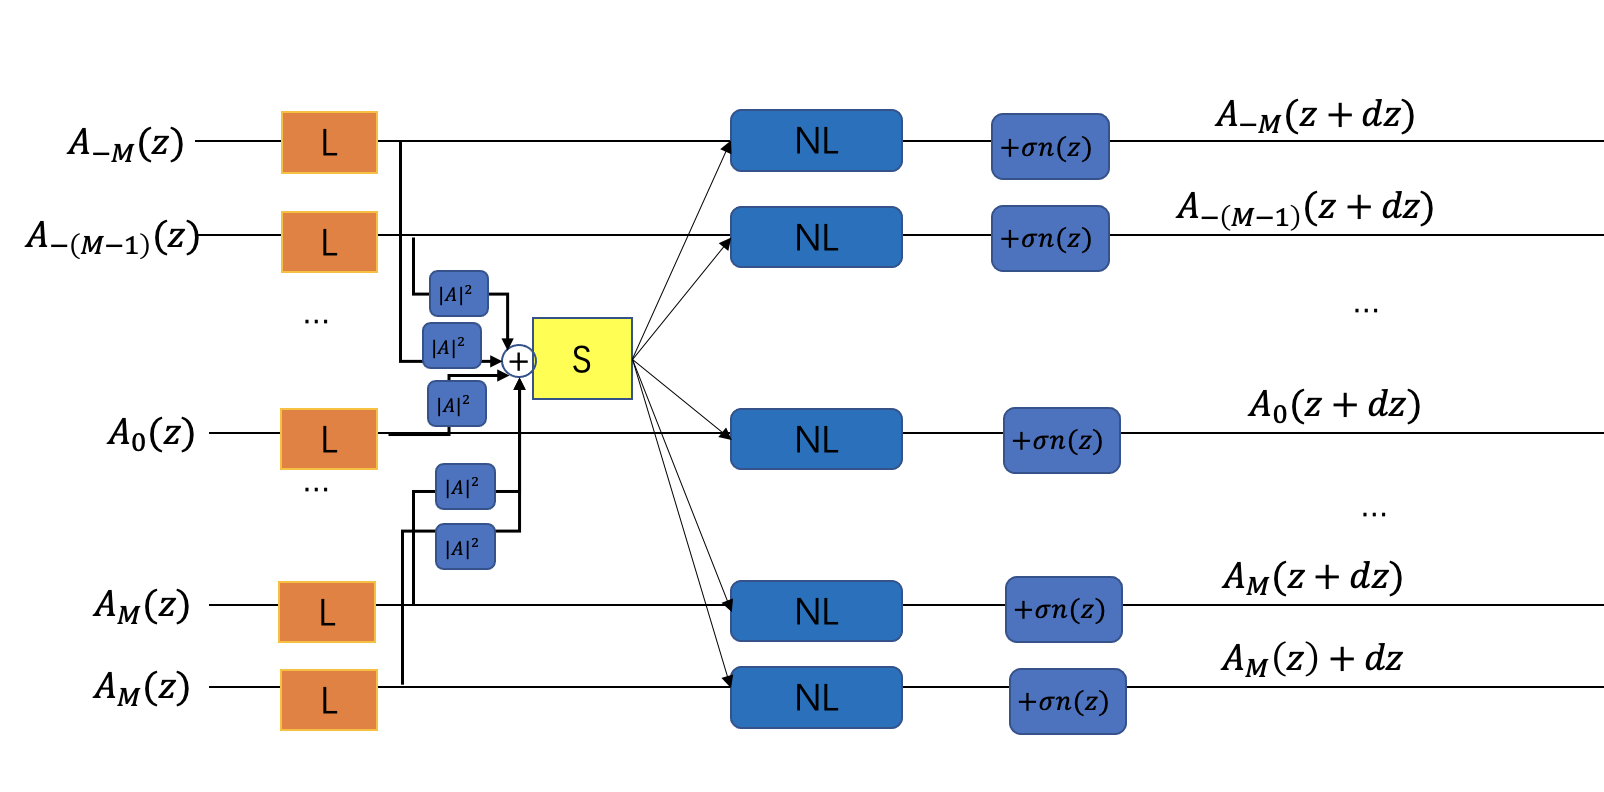
\includegraphics[width=0.6\linewidth]{img/SSFM.png}
\caption{SSFM structure: one step}
\label{SSFM fig}
\end{figure}
$$
SSFM: \left(\begin{array}{c}A_{-M}(0,t)\\A_{-(M-1)}(0,t)\\\ldots\\A_{0}(0,t)\\\ldots\\A_{M}(0,t)\end{array}\right) \rightarrow\left(\begin{array}{c}A_{-M}(L,t)\\A_{-(M-1)}(L,t)\\\ldots\\A_{0}(L,t)\\\ldots\\A_{M}(L,t)\end{array}\right)
$$
Using SSMF method: Linar step and Nonlinear step alternate. Assume each symbol take $N_t$ points sampling at equal intervals. Define collocation points $t_j = j\frac{T}{N_t} (0\leq j \leq N_{f})$. Here, $N_{f} = N*N_t$. 
\begin{align*}
A_i(z) := [A_i(z,t_0), A_i(z,t_1),\ldots,A_i(z,t_{N_{f}})] \in \mathbb{C}^{N_{f}} \\
\end{align*}
The transfer function:
\begin{align*}
& \mathbf{\omega} = \frac{2\pi}{T_f}[0,1,\ldots,\frac{N_f}{2},-\frac{N_f}{2}+1,-\frac{N_f}{2}+2,\ldots,-1] \in \mathbb{C}^{N_f}\\
& H_i(dz) = \exp \left[\left(-\frac{\alpha}{2} - \mathrm{i}\beta_{i1} \mathbf{\omega} - \mathrm{i} \beta_{i2} \frac{\mathbf{\omega}^{2}}{2}\right) dz\right] \in \mathbb{C}^{N_f}
\end{align*}
\begin{enumerate}
\item Linear step
\begin{equation}\label{linear step}
A_i(z + dz) = L_{H_i(dz)}(A_i(z)) := ifft(fft(A_i(z)) .* H_i(dz))
\end{equation}
\item Nonlinear step
\begin{equation}\label{nonlinear step}
A_i(z+dz) = NL_{dz,S_i} (A_i(z)) := A_i(z) .* \exp\left(\mathrm{i} \gamma dz * (S_i+|A_i|^2)\right) := A_i(z) .* \exp\left(i \gamma dz * (2\sum_{q\neq i} |A_q(z)|^2+|A_i(z)|^2)\right)
\end{equation}
We use $S_i$ to denotes the power sum of the other channels.
\begin{equation}\label{define S}
S_i = 2\sum_{q\neq i} |A_q(z)|^2
\end{equation}
\end{enumerate}

\begin{algorithm}[t]
\caption{SSFM} %算法的名字
\hspace*{0.02in} {\bf Input:} %算法的输入, \hspace*{0.02in}用来控制位置,同时利用 \\ 进行换行
input transmmitted signals $A_i(0)(-M \leq i \leq M)$, step size $dz$, noise level $\sigma$,transmmitted length $L$\\
\hspace*{0.02in} {\bf Output:} %算法的结果输出
output result
\begin{algorithmic}[1]
\State $K = \frac{L}{dz}$  % \State 后写一般语句
\For{s = 1,...,K} % For 语句,需要和EndFor对应
   \State Linear step:
        $$
        A_i^{1}(z) = L_{H_i(dz)}(A_i(z))
        $$
    \State Calculate $S_i$:
        $$
        S_i = 2\sum_{q\neq i} |A_i^1(z)|^2
        $$
    \State Nonlinear step:
        $$
        A_i^2(z) = NL_{dz,S_i}(A^1_i(z))
        $$
    \State Add noise: sample a gaussian noise $n(z)$.
        $$
            A_i(z+dz) \leftarrow A_i(z+dz) + \sigma * n(z)
        $$
    \State $z \leftarrow z + dz$
\EndFor
\State \Return $A_i(L)$, $-M \leq i \leq M$
\end{algorithmic}
\end{algorithm}
The whole process show in Figure [\ref{SSFM fig}].

\subsection{Receiver Model}
There are three steps in our receiver model.
\begin{enumerate}
\item Digital back propagation. This step is the most import part to compensate all kinds of interference. We will design some algorithm in Section 2.
    \begin{equation}\label{DBP}
    \hat{A}_0(t) = DBP(A_0(L,t))
    \end{equation}
\item Filter.
    \begin{equation}
    \tilde{x}_k^0 = \frac{1}{\sqrt{P_0} \|g\|_2^2}\int_{-\infty}^{+\infty} \hat{A}_0(t) g_k(t) dt
    \end{equation}
    Here we define $g_k(t) = g(t - kT)$, then $g_k$ is othorgonal with respect to diffrent $k$.
\item Classification.
    \begin{equation}
    \hat{x}_k^0 = \mathop{argmin}\limits_{x\in \mathcal{X}} \|x - \tilde{x}_k^0\|
    \end{equation}
\end{enumerate}
We can show the whole communication system as Figure \ref{communication system}.

\begin{figure}[htbp]
\centering
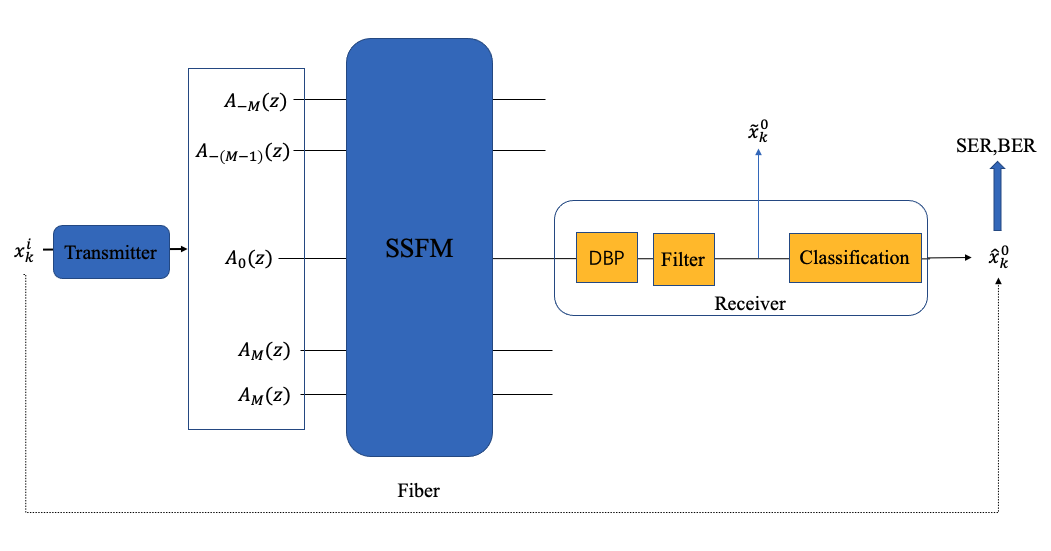
\includegraphics[width=0.8\linewidth]{img/com_system.png}
\caption{communication system}
\label{communication system}
\end{figure}














\section{Method:Digital back propagation}
This section aims to design the digital back propagation algorithm (See (\ref{DBP})). We concentrate on the central channel $A_0(z,t)$.
$$
DBP: A_0(L,t) \rightarrow \hat{A}_0(t)  
$$
The main challege is that we can not get the information of other channels. So we can not implement full channel digital propagation (FDBP).
We can construct several digital compensation method:

\subsection{Dispersion only DBP (DO-DBP)}
This method only compensate the linear distortion.
$$
\hat{A_0}(0) = L_{H_0(-L)}(A_0(L))
$$
\begin{figure}[htbp]
\centering
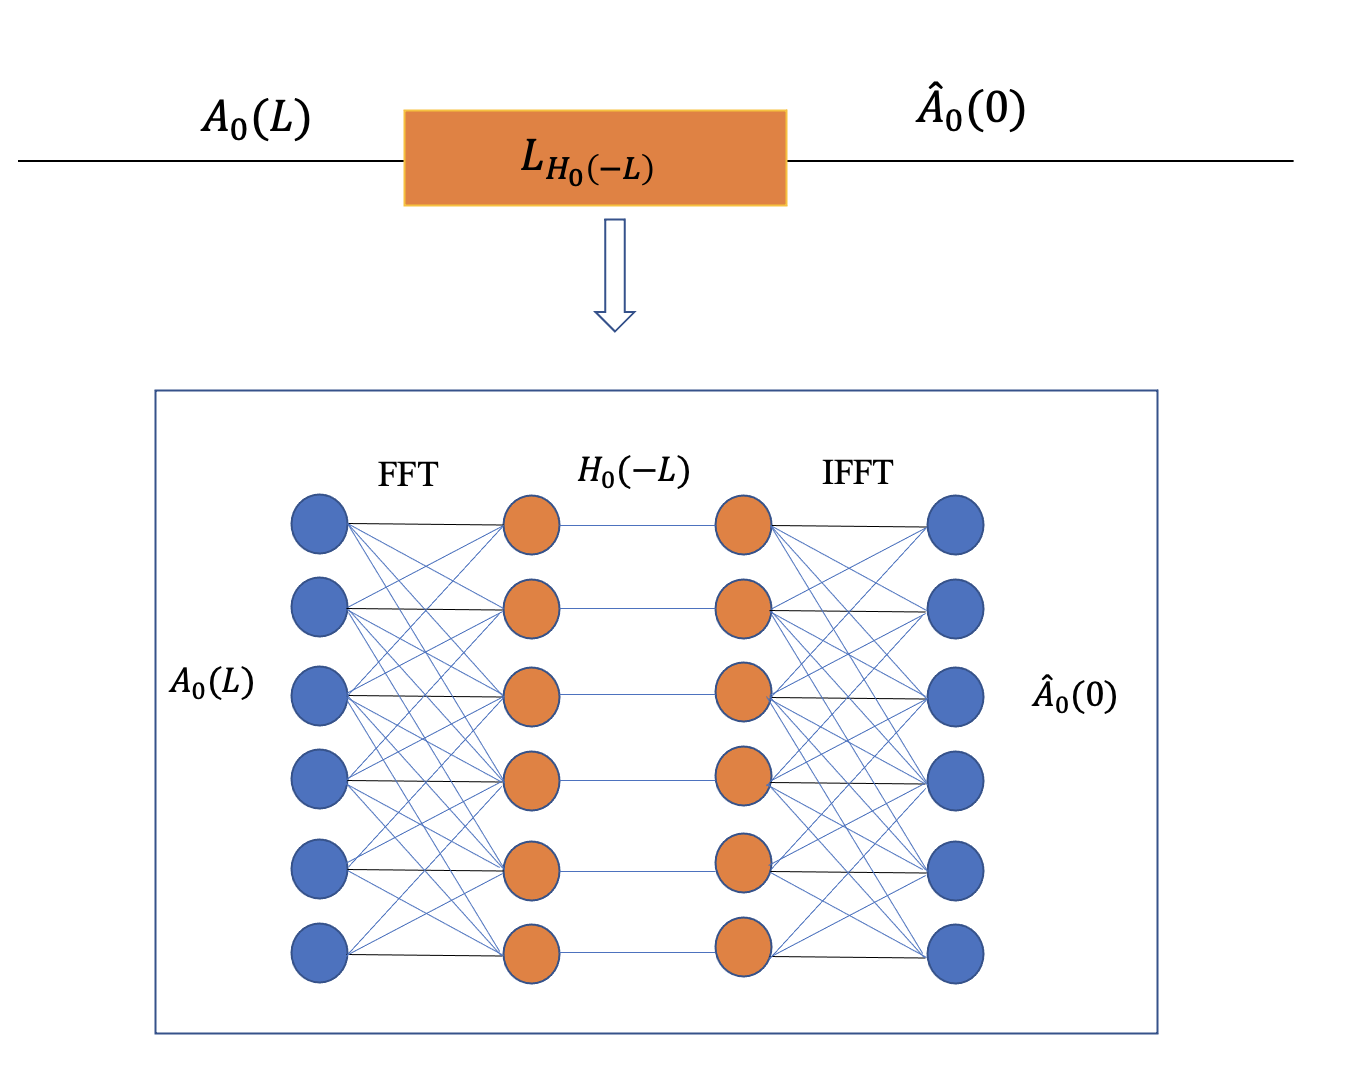
\includegraphics[width=0.6\linewidth]{img/DO-DBP.png}
\caption{Dispersion Only DBP}
\label{DO-DBP}
\end{figure}
\subsection{Single channel DBP (SC-DBP)}
$$
\hat{A}_0(0) = \left(\prod_{i=1}^{K} NL_{-dz,S_0=0} \circ L_{H_0(-dz)}\right)A_0(L,t)
$$
where K is $L/dz$ the span numbers. 
\begin{figure}[htbp]
  \centering
  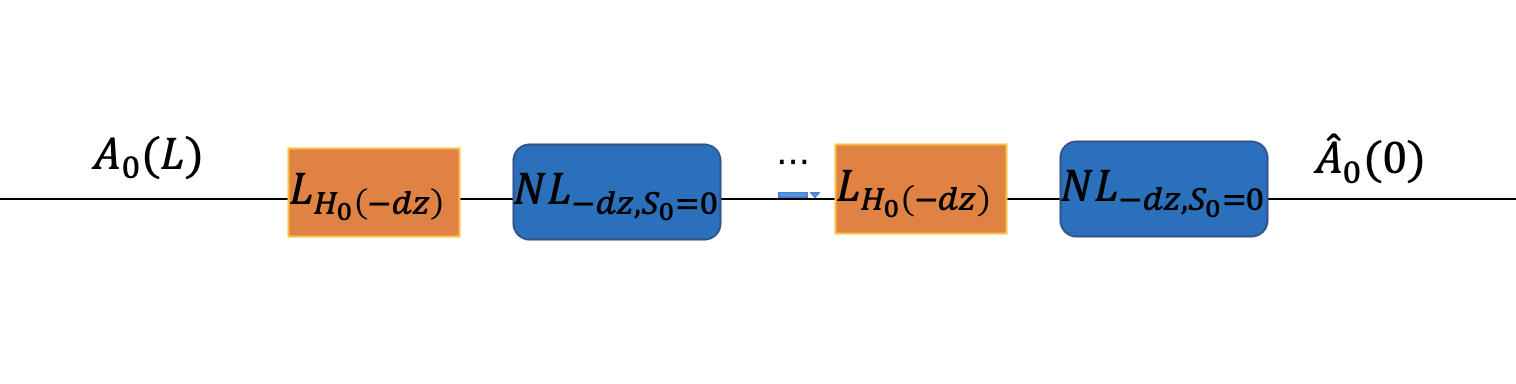
\includegraphics[width=0.6\linewidth]{img/SC-DBP.png}
  \caption{Single Channel DBP}
  \label{SC-DBP}
\end{figure}

\subsection{Neural Network DBP (NN-DBP)}
Notice that (\ref{linear step}) is a linear transform and (\ref{nonlinear step}) is a 
point wise nonlinear transform. SSFM are composed with Linear transform and nonlinear activations just like deep neural 
network.\cite{hager2020} and \cite{fan2020NC} find this similiar structure 
between SSFM and DNN. Set some parameters in SSFM to free then get NN-DBP. 
\begin{figure}[htbp]
\centering
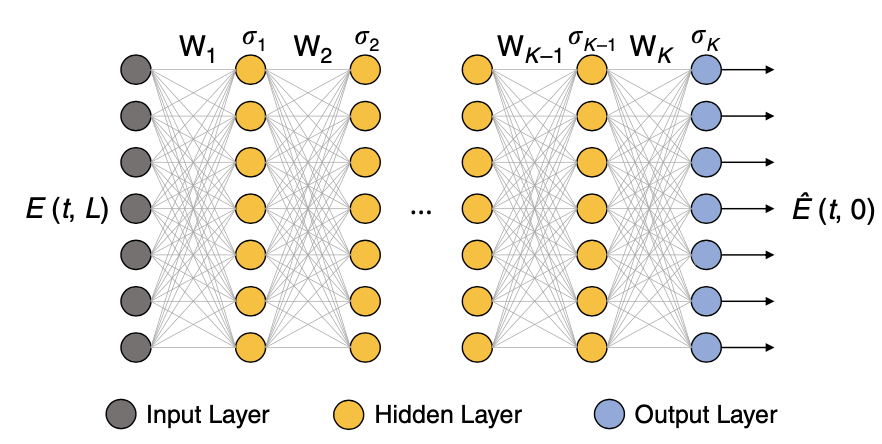
\includegraphics[width=0.6\linewidth]{img/NN.png}
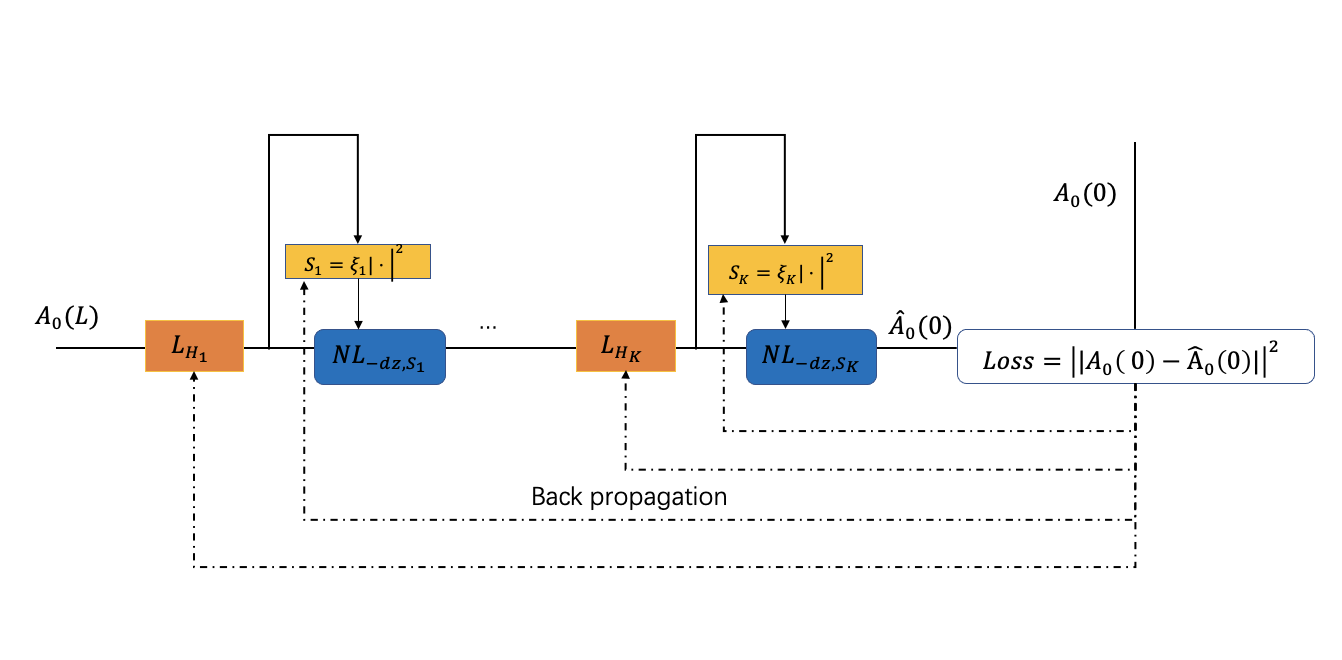
\includegraphics[width=0.6\linewidth]{img/NN-DBP.png}
\caption{NN structure \cite{fan2020NC}}
\label{NN}
\end{figure}
$$
D_i(u) = NL_{-dz,S_0 = \xi_i |u|^2} \circ L_{H_i}
$$
$$
\hat{A}(0) = \left(\prod_{i=1}^{K} D_i\right)A_0(L)
$$
where $\{\xi_i,H_i\}$ is the trained parameters.

$$
loss = \sum_{a_k^i \sim Uniform(\mathcal{X})} \|\hat{A}(0,t) - A(0,t)\|^2
$$

\subsection{Meta-1 DBP}
Use two fully connected networks to estimate $S_0$ and $H_0$ in each step. We want to guess some information
 from $A_0(L)$. This is a meta neural network.
\begin{equation}
S_0 = \phi(u,\theta_i), H_0 = \psi(u,\mu_i)
\end{equation}
$$
D_i(u) = \left(NL_{-dz,S_0=\phi(u;\theta_i)} \circ L_{H_0=\psi(u;\mu_i)}\right) (u)
$$

$$
\hat{A}(0,t) = \left(\prod_{i=1}^{K} D_i\right)A_0(L,t)
$$

where $\phi$ and $\psi$ is two fully connected networks, $\{\theta_i,\mu_i\}$ is the trained parameter. 

$$
loss = \sum_{a_k^i \sim Uniform(\mathcal{X})} \|\hat{A}(0,t) - A(0,t)\|^2
$$
\begin{figure}[htbp]
\centering
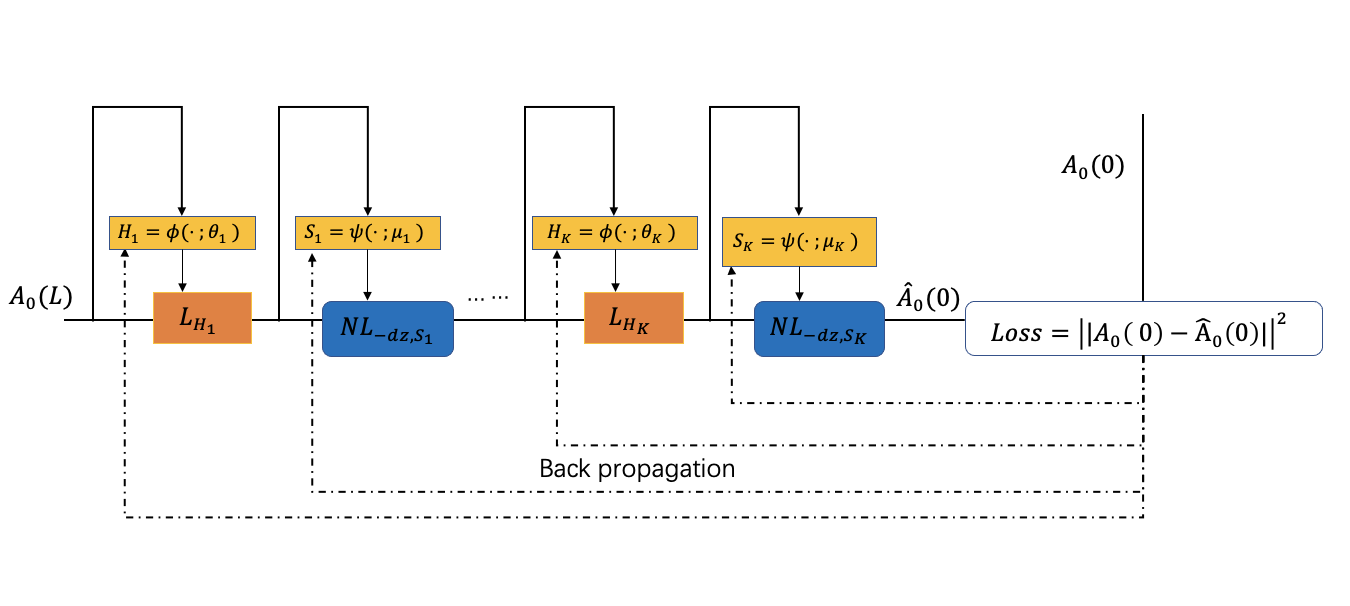
\includegraphics[width=0.6\linewidth]{img/Meta-1.png}
\caption{Meta-1 DBP structure}
\label{Meta-1}
\end{figure}

\begin{figure}[htbp]
  \centering
  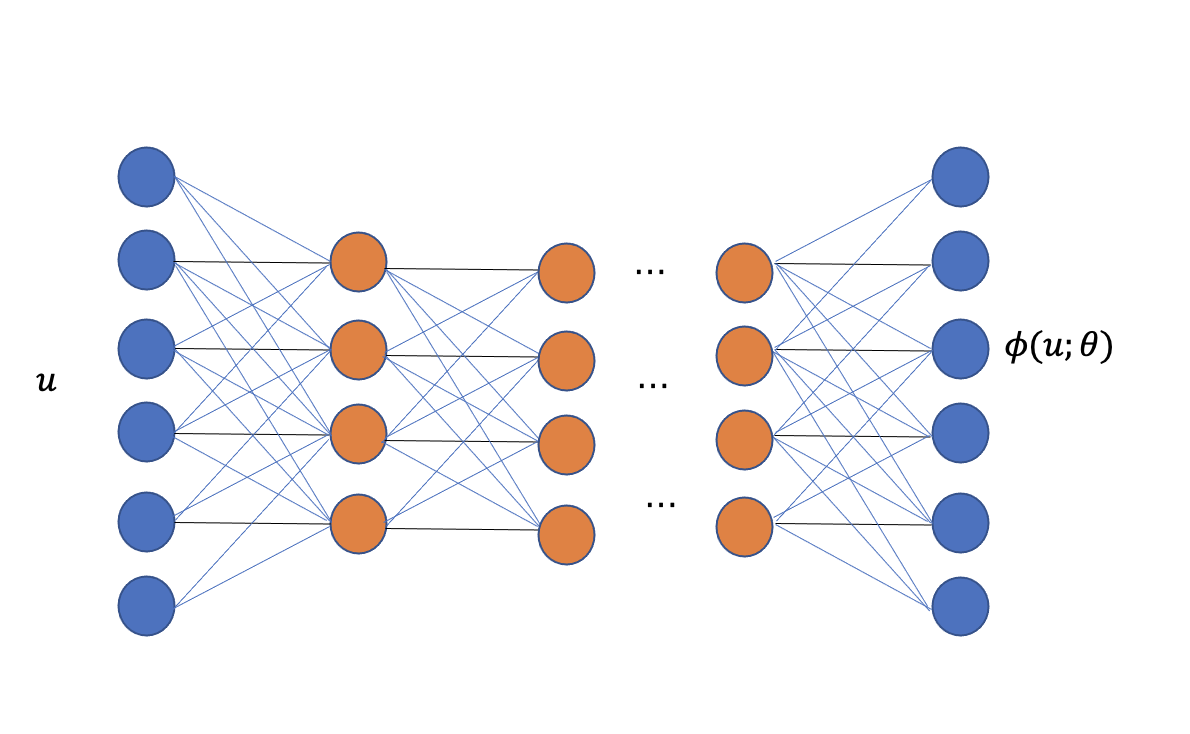
\includegraphics[width=0.4\linewidth]{img/FNNphi.png}
  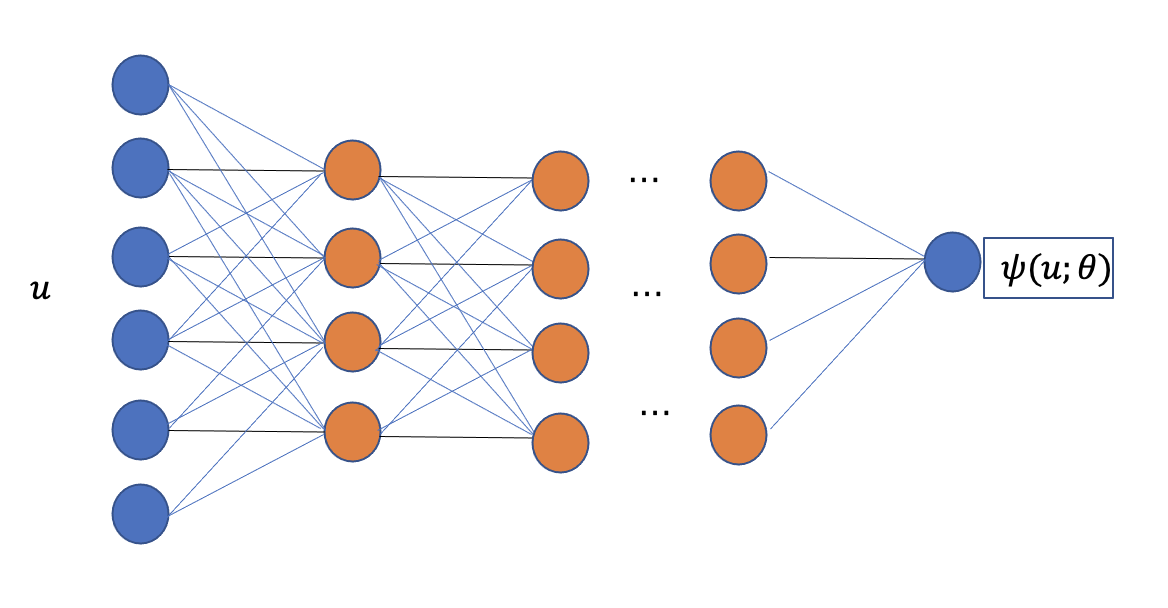
\includegraphics[width=0.4\linewidth]{img/FNNpsi.png}
  \caption{FNN structure}
  \label{FNN1}
  \end{figure}

\newpage
\subsection{Meta-2 DBP}
\begin{equation}
  S_0 = \phi(u,\theta_i)|u|^2, H_0 = \psi(u,\mu_i)
  \end{equation}
Change the meta form.
$$
D_i(u) = \left(NL_{-dz,S=\phi(u;\theta_i)|u|^2} \circ L_{-dz,H=\psi(u;\mu_i)}\right) (u)
$$

$$
\hat{A}(0,t) = \left(\prod_{i=1}^{K} D_i\right)A_0(L,t)
$$

where $\phi$ and $\psi$ is two fully connected networks, $\{\theta_i,\mu_i\}$ is the trained parameter. 

$$
loss = \sum_{a_k^i \sim Uniform(\mathcal{X})} \|\hat{A}(0,t) - A(0,t)\|^2
$$

\subsection{Meta-3 DBP}
Share the meta-net weight in different steps.
$$
D(u) = \left(NL_{-dz,S=\phi(u;\theta)} \circ L_{-dz,H=\psi(u;\mu)}\right) (u)
$$

$$
\hat{A}(0,t) = \left(\prod_{i=1}^{K} D_i\right)A_0(L,t)
$$

where $\phi$ and $\psi$ is two fully connected networks, $\{\theta,\mu\}$ is the trained parameter. 

$$
loss = \sum_{a_k^i \sim Uniform(\mathcal{X})} \|\hat{A}(0,t) - A(0,t)\|^2
$$

\section{Experiments result}
The details of experiment are showed in Table \ref{ex details}. We construct two training data sets.
\begin{enumerate}
  \item Data set A: $P_i = 50 [mW]$.
  \item Date set B: $P_i$ is i.i.d sampled from Uniform([50 mW,60 mW]) in each epoch.
\end{enumerate}
We use different widths and depths for A and B. See Table \ref{NN setting}. The loss curves are shown
in Figure \ref{loss}. Under setting A, we can see Meta-1 to Meta-3 can achive
better minimizers than NN-DBP. These methods converge steadily. Under Setting B, training becomes untractable.
The costellations are shown in Figure \ref{A fig} and \ref{B fig}. The BER results are shown in Table \ref{A table} and Table \ref{B table}.
We mainly consider comparation of 4 methods: NN-DBP,Meta-1,Meta-2,Meta-3.We can get conclusions as follows:
\begin{enumerate}
\item Under setting A:
\begin{itemize}
\item From the loss curve \ref{loss}, the four methods all converge smoothly, and the convergence point from Meta-1 to Meta-3 is better than NN-DBP. 
The loss curves of Meta-1 and Meta-2 almost overlap, which also shows a certain equivalence of the two methods. Meta-3 converges faster than Meta-1 and Meta-2, 
but the minimum point reached in the end is not as good as the first two.
\item From the costellation diagram \ref{A fig},when the test power is equal to the training power, the four methods all show the best results.When the test 
power is not equal to the training power, the non-linear phase shift is not perfectly compensated. Compared with the ideal result, there is a phase deflection overall
\item From table \ref{A table},when the test power is equal to 50mW, Meta-1 to Meta-3 are better than NN-DBP by about $2\%$. 
Other test power performances are not good, and there is no comparative value.
没有比较价值。
\end{itemize}
\item Under setting B:(Since Meta-1 and Meta-2 behave very similarly in A, the Meta-2 experiment was omitted here.)
\begin{itemize}
\item From the loss curve \ref{loss}, the convergence of the four methods is very difficult. Meta-1 is better than Meta-3. Meta-3 is better than NN-DBP
\item From the constellation diagram, when test power = 55mW, the four methods perform best. Other power values behave similarly to A, with a phase rotation difference overall. This means neural network
Learned an average power result in the training set. This also shows that our method is invalid without knowing the power of the interfering channel
\item From table \ref{A table},when the test power is equal to 55 mW, Meta-1 and Meta-3 are better than NN-DBP by about $2\%$. 
Other test power performances are not good, and there is no comparative value.
\end{itemize}
\end{enumerate}

\begin{table}[htbp]
  \centering
  \begin{tabular}{lll}
    \hline
    setting       & width & depth \\
    \hline
    A           &  60   &   2   \\
    \hline
    B           &  120  &   3   \\
    \hline
  \end{tabular}
  \caption{experiments details}
  \label{NN setting}
\end{table}

\begin{table}[htbp]
  \centering
  \begin{tabular}{llll}
  parameter        & variable  & quantity & unit \\
  \hline
  attenuation      & $\alpha$  &   0.2     &  [dB/km]  \\
  \hline
  dispersion       & $\beta_2$ &   -21.68  &   [$ps^2 km^{-1}$]   \\
  \hline
  nonlinear        & $\gamma$  &   1.37   &  [$W^{-1} km^{-1}$]   \\
  \hline
  peak power       & $P_0$     &   50     &  [mW] \\
  \hline
  number of WDM channel& $2M+1$  &    3   &   1 \\
  \hline
  length of fiber  & L         &     100   & [km] \\
  \hline
  symbol rate      & $R_s = \frac{1}{T_f}$ & 10 & [GHz]\\
  \hline
  central wavelength & $\lambda_0$ & 1550  & [nm] \\
  \hline
  channel space      &   $\Delta \lambda $     & 0.4   & [nm] \\
  \hline 
  roll              & $\beta$     & 0.2 & 1 \\
  \hline
  noise level       & $\sigma$    & 0.002 & 1 \\
  \hline
  number of symbols  & N          & 128   & 1 \\
  \hline
  number of samples/symbol & $N_t$ & 8    & 1 \\
  \hline
  \end{tabular}
  \caption{experiments details}
  \label{ex details}
\end{table}


\begin{figure}[htbp]
  \centering
  \subfigure[Loss curve for Data set A]{
    \begin{minipage}[t]{0.4\linewidth}
      \centering
      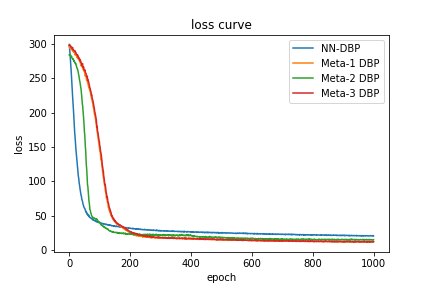
\includegraphics[width=0.9\linewidth]{img/expriment/fixpower_loss.png}
    \end{minipage}
  }
  \subfigure[Loss curve for Data set B]{
    \begin{minipage}[t]{0.4\linewidth}
      \centering
      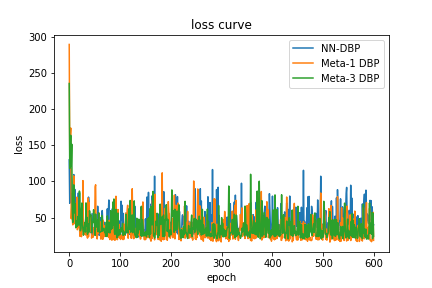
\includegraphics[width=0.9\linewidth]{img/expriment/W120-D3-loss.png}
    \end{minipage}
  }
  \caption{Loss curve for Data set A and B}
  \label{loss}
  \end{figure}


  
  \begin{figure}[htbp]
  \centering
  \subfigure[test power: 50mW]{
    \begin{minipage}[t]{0.8\linewidth}
      \centering
      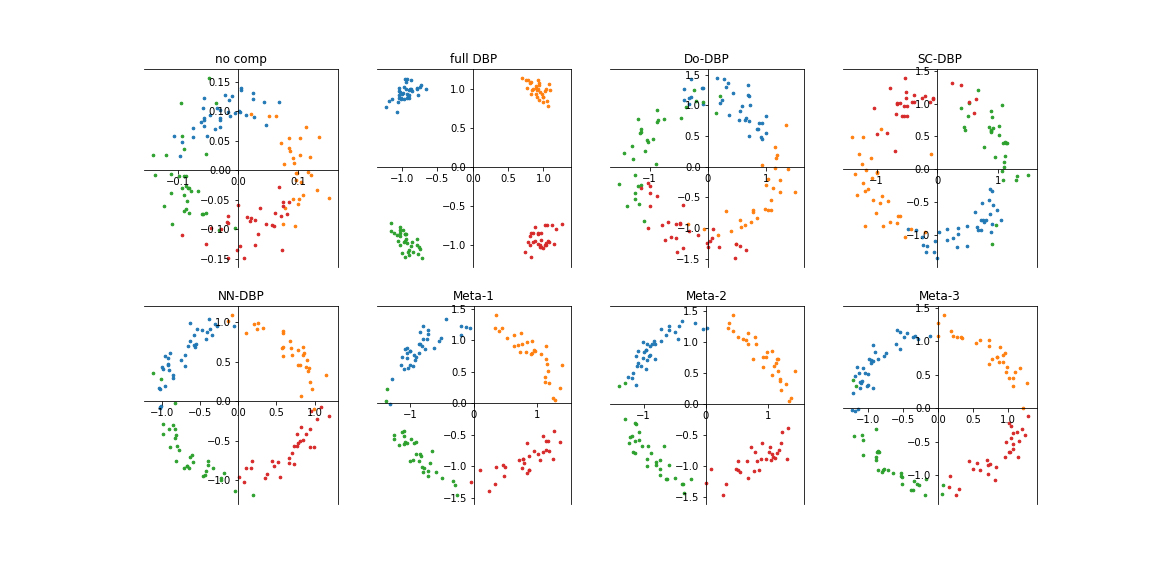
\includegraphics[width=1\linewidth]{img/expriment/W60-D2-P50star.png}
    \end{minipage}
  }
  
  \subfigure[test power: 55 mW]{
    \begin{minipage}[t]{0.8\linewidth}
      \centering
      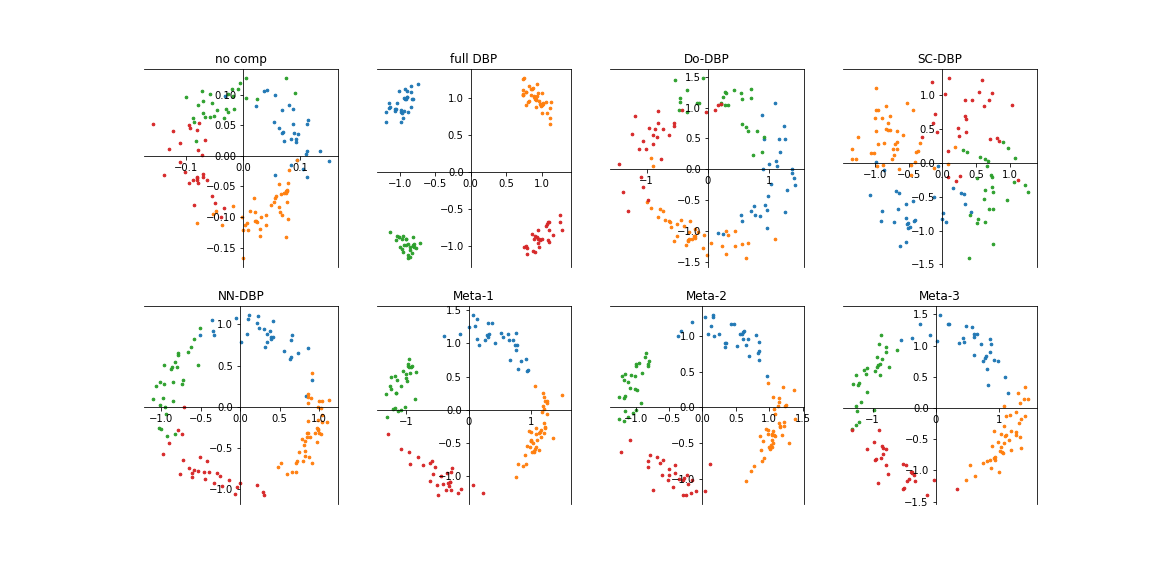
\includegraphics[width=1\linewidth]{img/expriment/W60-D2-P55star.png}
    \end{minipage}
  }
  
  \subfigure[test power: 45 mW]{
    \begin{minipage}[t]{0.8\linewidth}
      \centering
      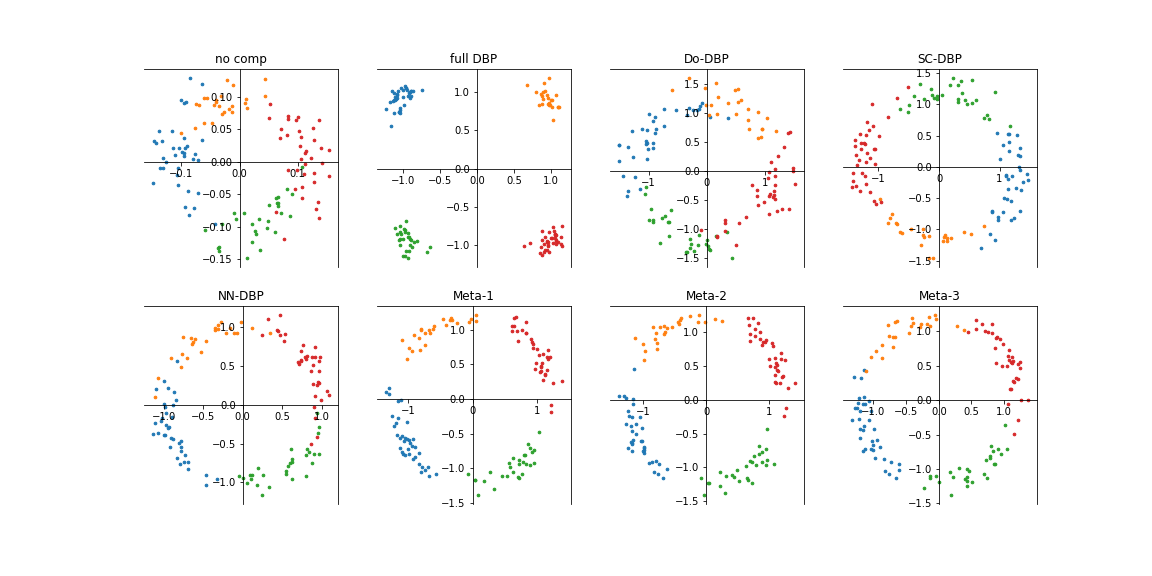
\includegraphics[width=1\linewidth]{img/expriment/W60-D2-P45star.png}
    \end{minipage}
  }
  \caption{Plot the $\tilde{x}_k^0$. Training with Data Set A.  Test with power: 50[mW],52[mW], 45[mW]}
  \label{A fig}
  \end{figure}


\begin{table}[htbp]
\centering
\begin{tabular}{llll}
\hline
\multicolumn{2}{l}{Test power: 50[mW]} & Test power: 52[mW] & Test power: 45[mW] \\
\hline
Method & Acc(100 times mean)  & Acc(100 times mean)  & Acc(100 times mean)\\
    DO-DBP  &  0.586914   &    0.421367  &    0.9275  \\
    SC-DBP  &  0.0989844  &   0.216875  &   0.12375 \\
    NN-DBP  &  0.963242   &   0.886992  &   0.573984 \\
    Meta-1  &  0.989297   &   0.910117   &   0.559688 \\
    Meta-2  &  0.984766   &   0.895469   &   0.556758 \\
    Meta-3  &  0.975234   &   0.893203 &   0.589961 \\
    \hline
\end{tabular}
\caption{Test result. Training data: A}
\label{A table}
\end{table}

\begin{table}[htbp]
  \centering
  \begin{tabular}{ll}
  \hline
  \multicolumn{2}{l}{Test power: 50[mW]}\\
  Method    &    BER    \\
   no comp  &   0.518125 \\
  full DBP  &   0 \\
    DO-DBP  &   0.334219 \\
    SC-DBP  &   0.381836 \\
    NN-DBP  &   3.08594e-05 \\
    Meta-1  &   2.73437e-06 \\
    Meta-2  &   1.5625e-06 \\
    Meta-3  &   1.01563e-05 \\
      \hline
  \end{tabular}
  \caption{TEST}
  \label{test test}
  \end{table}

\begin{table}[htbp]
  \centering
  \begin{tabular}{llll}
  \hline
  \multicolumn{2}{l}{Test power: 50[mW]} & Test power: 55[mW] & Test power: 60[mW] \\
  \hline
  Method & Acc(100 times mean)   & Acc(100 times mean)  & Acc(100 times mean)\\
      DO-DBP  &  0.587461  &   0.170586  &   0.318281 \\
      SC-DBP  &   0.0934766  &   0.410273  &    0.652031 \\
      NN-DBP  &   0.594141 &   0.948281  &   0.635977\\
      Meta-1  & 0.600195 &    0.974766  &    0.606836\\
      Meta-3  &  0.603828  &    0.964063  &   0.601992 \\
      \hline
  \end{tabular}
  \caption{Test result. Training data: B}
  \label{B table}
  \end{table}

\begin{figure}[htbp]
\centering
\subfigure[test power: 50mW]{
  \begin{minipage}[t]{0.8\linewidth}
    \centering
    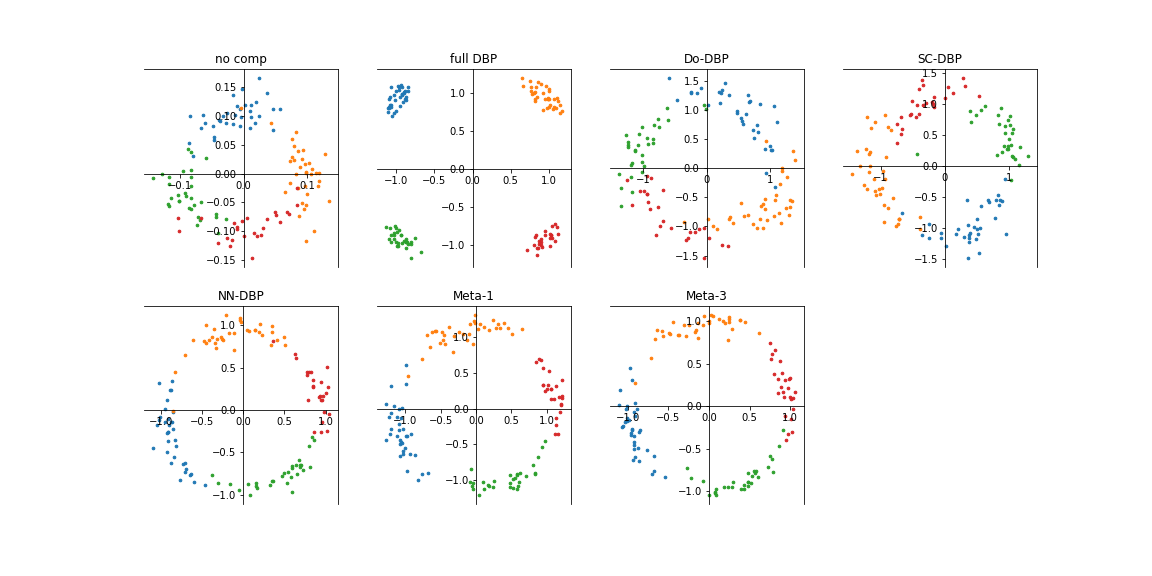
\includegraphics[width=1\linewidth]{img/expriment/W120-D3-P50star.png}
  \end{minipage}
}

\subfigure[test power: 55 mW]{
  \begin{minipage}[t]{0.8\linewidth}
    \centering
    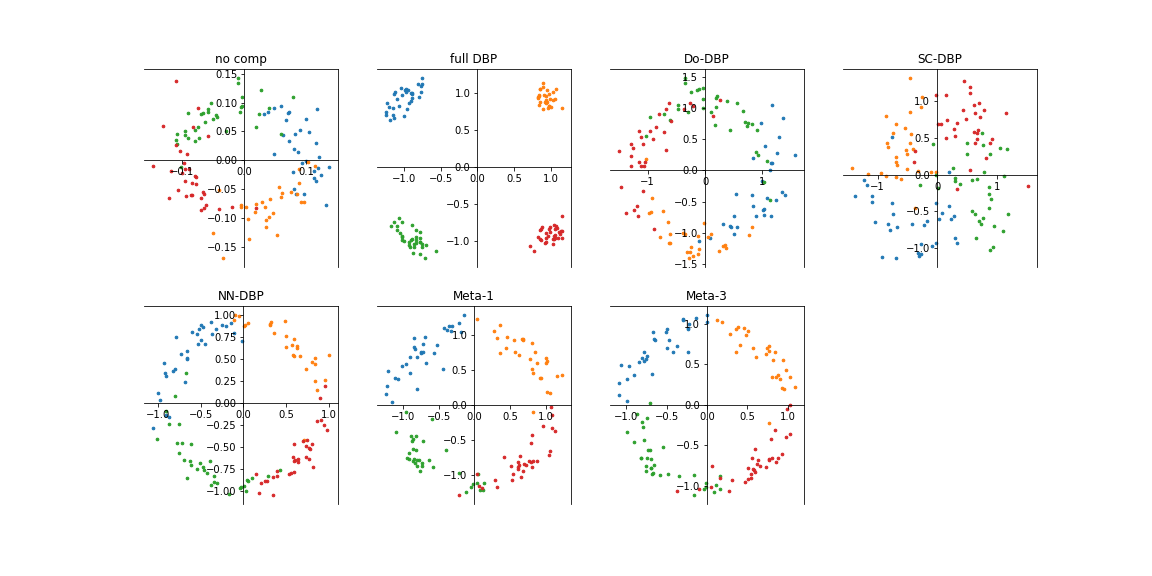
\includegraphics[width=1\linewidth]{img/expriment/W120-D3-P55star.png}
  \end{minipage}
}

\subfigure[test power: 60 mW]{
  \begin{minipage}[t]{0.8\linewidth}
    \centering
    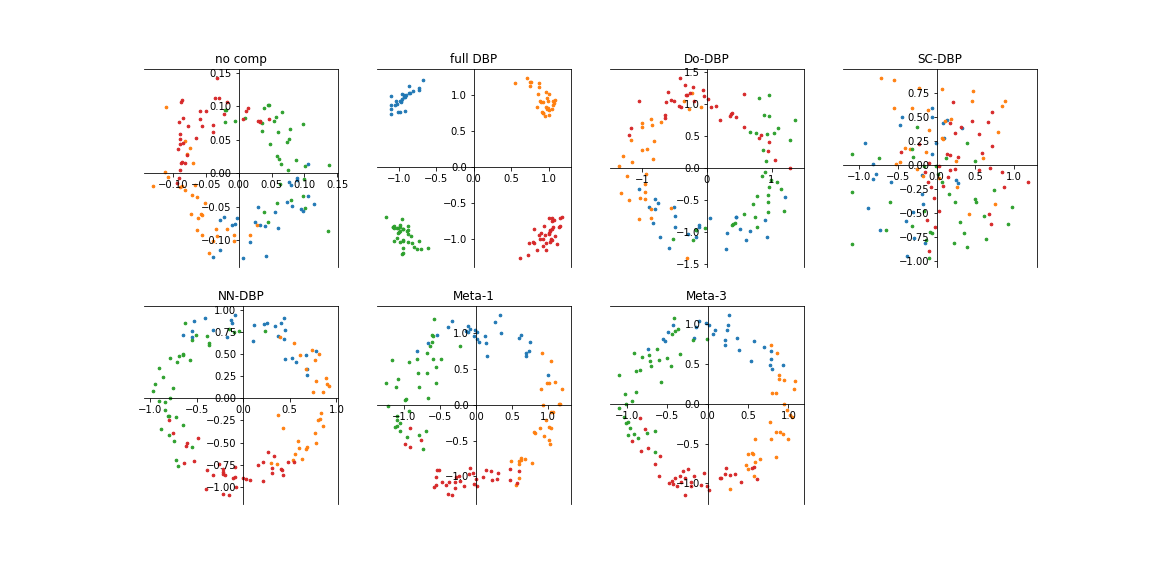
\includegraphics[width=1\linewidth]{img/expriment/W120-D3-P60star.png}
  \end{minipage}
}
\caption{Plot the $\tilde{x}_k^0$. Training with data set B, Test with power: 50[mW],55[mW],60[mW]}
\label{B fig}
\end{figure}

\newpage
\section{Future work}
\begin{enumerate}
\item Improve the Meta-NN structure. Use CNN,RNN etc. Test the boundary of our method.
\item Use the data from physical experiment.(Thank Qiri Fan(author of \cite{fan2020NC}) for provding the data).
\item Consider simulating the optical pulse propagation with Vector Manakov–PMD equation.
$$
\begin{aligned}
\frac{\partial \Psi}{\partial z}=&\left(-\frac{1}{2} \alpha-j \boldsymbol{\beta}_{0}-\boldsymbol{\beta}_{1} \frac{\partial}{\partial t}-j \beta_{2} \frac{1}{2} \frac{\partial^{2}}{\partial t^{2}}\right) \Psi 
&+j \frac{8}{9} \gamma|\boldsymbol{\Psi}|^{2} \boldsymbol{\Psi}+\left[\begin{array}{l}
n_{x}(z, t) \\
n_{y}(z, t)
\end{array}\right]
\end{aligned}
$$
\item Change the system parameter to approach real optical fiber system. In particular, increase 
symbol rate to 60 [GHz]. Increase number of spans to about 10. Change the distributed noise to EDFA noise.
Reduce peak power to about 1[mW]. Increase number channels. The most important thing is to think about how
to pose the problem. Under what circumstances can it be resolved, and under what circumstances will it reach the unsolvable boundary。
\item Improve the structure of the transmitter and receiver, set reasonable down sampling rules, and add some classic adaptive filters and adaptive phase noise estimators (FOE, CPE) to improve
System performance.
\item Considering the calculation limitations of practical applications, balance calculation performance and accuracy improvement.
\end{enumerate}



\section{Digital Signal Processing Basics}

\subsection{Polarization model dispersion}
Basic relationships in vacuum:
\begin{equation}
\lambda f = c, \omega = 2\pi f, k = \frac{2\pi}{\lambda} = \frac{\omega}{c}
\end{equation}
\begin{table}[htbp]
    \centering
    \begin{tabular}{lll}
    physic        & variable  & unit \\
    \hline
    wave length   & $\lambda$ &  [m]  \\
    \hline
    frequency    &  f         & Hz \\ 
    \hline
    angular frequency & $\omega$ & [rads/s] \\
    \hline
    wave number    &   k        &  [rads/m] \\
    \hline
    \end{tabular}
    \caption{physical variable}
    \label{physical variable}
\end{table}
When a beam of light goes into fiber, its frequency remains the same, wavelength changes, then its velocity 
changes.
$$
v(\omega) = \frac{c}{n(\omega)}
$$
\begin{equation}
\lambda f = v(\omega), \omega = 2\pi f, \beta = \frac{2\pi}{\lambda} = \frac{\omega}{v(\omega)} = \frac{n(\omega)\omega}{c}
\end{equation}

In real fibers, small departures from cylindrical symmetry, 
occurring because of random variations in the core shape along the fiber length, 
result in a mixing of the two polarization states by breaking the mode degeneracy.
Mathematically, the mode-propagation constant $\beta$ becomes slightly different for the modes polarized in the x and
y directions.  This property is referred to as modal birefringence.  The strength of modal
birefringence is defined by a dimensionless parameter.
$$
B_{m}=\frac{\left|\beta_{x}-\beta_{\gamma}\right|}{k_{0}}=\left|n_{x}-n_{\gamma}\right|
$$
beat length:
$$
L_{B}=\frac{2 \pi}{\left|\beta_{x}-\beta_{y}\right|}=\frac{\lambda}{B_{m}}
$$


\subsection{Coherent detection}
We use a electronic field to describe light:
$$
\mathbf{E}(z, t)=\mathbf{E}_{0} e^{i(k z-2 \pi f t)}=\left(\hat{x} E_{0 x}+\hat{y} E_{0 u}\right) e^{i(k z-2 \pi f t)}
$$
We use a Jones vector to describe a polarization state of light.

We consider Homodyne Receiver
$$
E_s(t) = A_s(t) exp(j\omega_s t)
$$

\subsection{Adaptive filter theory}



Some DSP techniques need to learn:
\begin{itemize}
    \item Coherent receiver
    \item FDBP (filter DBP)
    \item FOE (Frequency offset estimater)
    \item BPM (Batch power normalization)
    \item MIMO (Multi Input Multi Output)
    \item CPE (carrier phase estimator)
\end{itemize}

Problems to derive:
\begin{itemize}
    \item NLSE -- CNLSE
\end{itemize}


\section{Jax Programming}







\newpage
\printbibliography{}
\end{CJK}
\end{document}